\documentclass{standalone}
\usepackage[ngerman]{babel}
% https://tex.stackexchange.com/questions/570303/use-blacktriangleright-as-itemize-label
\usepackage{amssymb} % for black triangleright

\renewcommand{\labelitemi}{$\textcolor{SwitchColor}{\bullet}$}
\renewcommand{\labelitemii}{$\textcolor{SwitchColor}{\blacktriangleright}$}
\renewcommand{\labelitemiii}{$\textcolor{SwitchColor}{\blacksquare}$}

% https://tex.stackexchange.com/questions/525959/prevent-latex-from-stretching-math
\setlength{\thinmuskip}{1\thinmuskip}
\setlength{\medmuskip}{1\medmuskip}
\setlength{\thickmuskip}{1\thickmuskip}

\usepackage{array}
\usepackage{booktabs}
\usepackage{boldline}

\usepackage{csquotes}
\usepackage{xcolor}
% \usepackage{anyfontsize}
\usepackage[export]{adjustbox}
% \usepackage[]{enumitem}
\usepackage{nicematrix}
\usepackage{tikz}
\usetikzlibrary{arrows.meta,positioning}
\usetikzlibrary{graphs}
\usetikzlibrary{patterns}
\usetikzlibrary{shadings}
\usetikzlibrary{mindmap, shadows, backgrounds} % , calc

\definecolor{PrimaryColor}{HTML}{0B64A0}
\definecolor{PrimaryColorDimmed}{HTML}{A2D7F3}
\definecolor{SecondaryColor}{HTML}{6FC1EC}
\definecolor{SecondaryColorDimmed}{HTML}{CEEAF9}
\colorlet{BoxColor}{gray!10!white}

% colored bold
% \newcommand\alert[1]{\textcolor{SwitchColor}{\textbf{#1}}}
\newcommand\alert[1]{\textcolor{SwitchColor}{#1}}

\newlength{\leveldistance}
\setlength{\leveldistance}{25cm}

\begin{document}
  \begin{tikzpicture}[
      auto,
      huge mindmap,
      fill opacity=0.6,
      draw opacity=0.8,
      concept color = PrimaryColorDimmed,
      every annotation/.style={fill=BoxColor, draw=none, align=center, fill = BoxColor, text width = 2cm},
      grow cyclic,
      level 1/.append style = {
        concept color=SecondaryColorDimmed,
        level distance=\leveldistance,
        sibling angle=360/\the\tikznumberofchildren,
        % https://tex.stackexchange.com/questions/501240/trying-to-use-the-array-environment-inside-a-tikz-node-with-execute-at-begin-no
        execute at begin node=\definecolor{SwitchColor}{named}{SecondaryColor},
      },
      level 2/.append style = {
        concept color=PrimaryColorDimmed,
        level distance=\leveldistance / 2,
        sibling angle=30,
        execute at begin node=\definecolor{SwitchColor}{named}{PrimaryColor},
      },
      level 3/.append style = {
        concept color=SecondaryColorDimmed,
        level distance=\leveldistance / 3,
        execute at begin node=\definecolor{SwitchColor}{named}{SecondaryColor},
      },
      level 4/.append style = {
        concept color=PrimaryColorDimmed,
        level distance=\leveldistance / 4,
        execute at begin node=\definecolor{SwitchColor}{named}{PrimaryColor},
      },
      level 5/.append style = {
        concept color=SecondaryColorDimmed,
        level distance=\leveldistance / 5,
        execute at begin node=\definecolor{SwitchColor}{named}{SecondaryColor},
      },
      level 6/.append style = {
        concept color=PrimaryColorDimmed,
        level distance=\leveldistance / 6,
        execute at begin node=\definecolor{SwitchColor}{named}{PrimaryColor},
      },
      level 7/.append style = {
        concept color=SecondaryColorDimmed,
        level distance=\leveldistance / 7,
        execute at begin node=\definecolor{SwitchColor}{named}{SecondaryColor},
      },
      level 8/.append style = {
        concept color=PrimaryColorDimmed,
        level distance=\leveldistance / 8,
        execute at begin node=\definecolor{SwitchColor}{named}{PrimaryColor},
      },
      concept connection/.append style = {
        color = BoxColor,
      },
  ]
  % damit Annotationen nicht auch eine Drop Shadow erhalten
  \begin{scope}[
      every node/.style = {concept, circular drop shadow}, % draw=none
      every child/.style={concept},
    ]
  \node (ca) at (current page.center) {Technische Informatik}
    child {
      node {Kodierung von Zeichen}
      child {
        node {Code, Codewörter
          \resizebox{\textwidth}{!}{
            \begin{minipage}[t]{10cm}
              \begin{itemize}
                \item Menge der \alert{Codewörter}: $c(A):=\left\{w\in\{0,1\}^{*}\;\right|\exists a\in A:c(a)=w\}$
                \item Eine Abbildung $c:{A}\rightarrow\{0,1\}^{*}$ oder $c:A\to\{0,1\}^{n}$ heißt \alert{Code}, falls $c$ injektiv ist 
              \end{itemize}
            \end{minipage}
          }
        }
        child {
          node {Alphabete, Wörter, Zeichen
            \resizebox{\textwidth}{!}{
              \begin{minipage}[t]{10cm}
                \begin{itemize}
                  \item nichtleeres Menge $A=\left\{a_{1},\dots,a_{m}\right\}$ heißt (endliches) \alert{Alphabet} der Größe $m$
                  \begin{itemize}
                    \item $a_1,\ldots, a_m$ heißen \alert{Zeichen} des Alphabets
                    \item $A^{*}=\{w\mid w=b_{1}\dots b_{n}\;m i t\;n\in\mathbb{N},\forall i\;m i t\;1\leq i\leq n:b_{i}\in A\}$ ist die \alert{Menge aller endlichen Wörter} über dem Alphabet $A$
                    \item $|b_1\ldots b_n| := n$ heißt Länge des Wortes $b_1\ldots b_n$
                    \item das Wort der Länge $0$ wird mit $\epsilon$
                  \end{itemize}
                \end{itemize}
              \end{minipage}
            }
          }
        }
        child {
          node {Codes fester Länge
            \resizebox{\textwidth}{!}{
              \begin{minipage}[t]{10cm}
                \begin{itemize}
                  \item $c:A\to\{0,1\}^{n}$ heißt \alert{Code fester Länge}
                  \begin{itemize}
                    \item für einen Code $c:A\to\{0,1\}^{n}$ fester Länge gilt: $n \ge \lceil log_2(m)\rceil$
                    \item ist $n=\lceil log_{2}m\rceil+r$ mit $r > 0$, so können die $r$ zusätzlichen Bits zum Test auf \alert{Übertragungsfehler} verwendet werden
                    \item Die Kodierung eines jeden Zeichens besteht aus $n$ Bits
                  \end{itemize}
                \end{itemize}
              \end{minipage}
            }
          }
          child {
            node {ASCII
              \resizebox{\textwidth}{!}{
                \begin{minipage}[t]{8cm}
                  \begin{itemize}
                    \item American Standard Code for Information Interchange
                    \item 7 Bits (es gibt Erweiterungen mit 8 Bits)
                  \end{itemize}
                  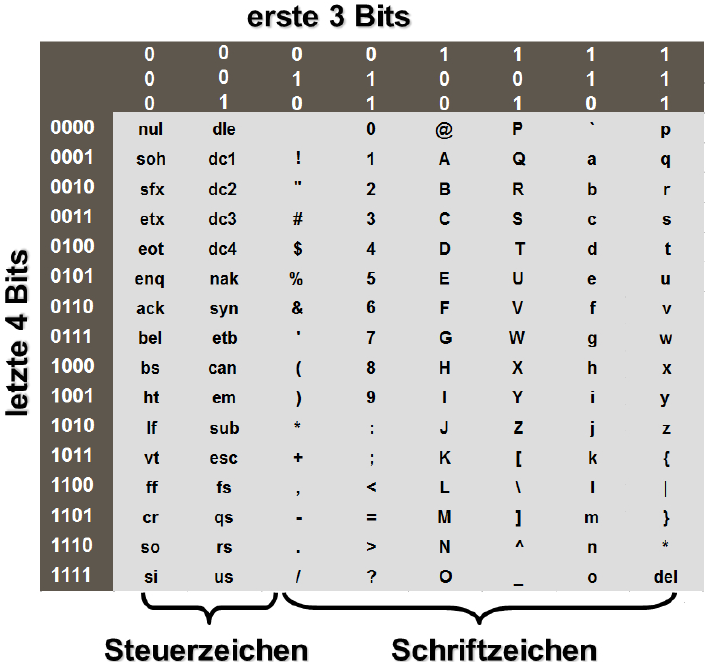
\includegraphics[width=0.5\textwidth, center]{./figures/ascii.png}
                \end{minipage}
              }
            }
          }
          child {
            node {EBCDIC
              \resizebox{\textwidth}{!}{
                \begin{minipage}[t]{8cm}
                  \begin{itemize}
                    \item Extended Binary Coded Decimal Interchange Code
                    \item 8 Bits
                  \end{itemize}
                \end{minipage}
              }
            }
          }
          child {
            node {Unicode
              \resizebox{\textwidth}{!}{
                \begin{minipage}[t]{8cm}
                  \begin{itemize}
                    \item 16 Bits
                  \end{itemize}
                \end{minipage}
              }
            }
          }
        }
        child {
          node {Häufigkeits-abhängige Codes
            \resizebox{\textwidth}{!}{
              \begin{minipage}[t]{8cm}
                \begin{itemize}
                  \item \alert{Ziel} ist die Reduktion der Länge einer Nachricht durch Wahl \alert{verschieden lange Codewörter} für die verschiedenen Zeichen eines Alphabets
                  \item häufiges Zeichen $\rightarrow$ kurzer Code
                  \item seltenes Zeichen $\rightarrow$ langer Code
                  % \item Häufigkeitsverteilung ist bekannt $\rightarrow$ \alert{statische Kompression}
                  % \item Häufigkeitsverteilung ist nicht bekannt $\rightarrow$ \alert{dynamische Kompression}
                \end{itemize}
              \end{minipage}
            }
          }
            child {
              node {Huffman
                \resizebox{\textwidth}{!}{
                  \begin{minipage}[t]{10cm}
                    \begin{itemize}
                      \item \alert{Vorgehen:}
                      \begin{enumerate}
                        \item Baue binären Baum, indem die beiden kleinsten Häufigkeiten jeweils zu einem neuen Knoten addiert werden
                        \item Markiere die linken Kanten mit $0$ und die rechten Kanten mit $1$, fertig ist der Huffman-Code
                      \end{enumerate}
                      \item Huffman-Code ist ein bzgl. mittlerer Codelänge optimaler \alert{Präfixcode} (unter Voraussetzung einer bekannten Häufigkeitsverteilung)
                      \item Kommt als Teilschritt z.B. in MP3 oder JPEG vor.
                    \end{itemize}
                    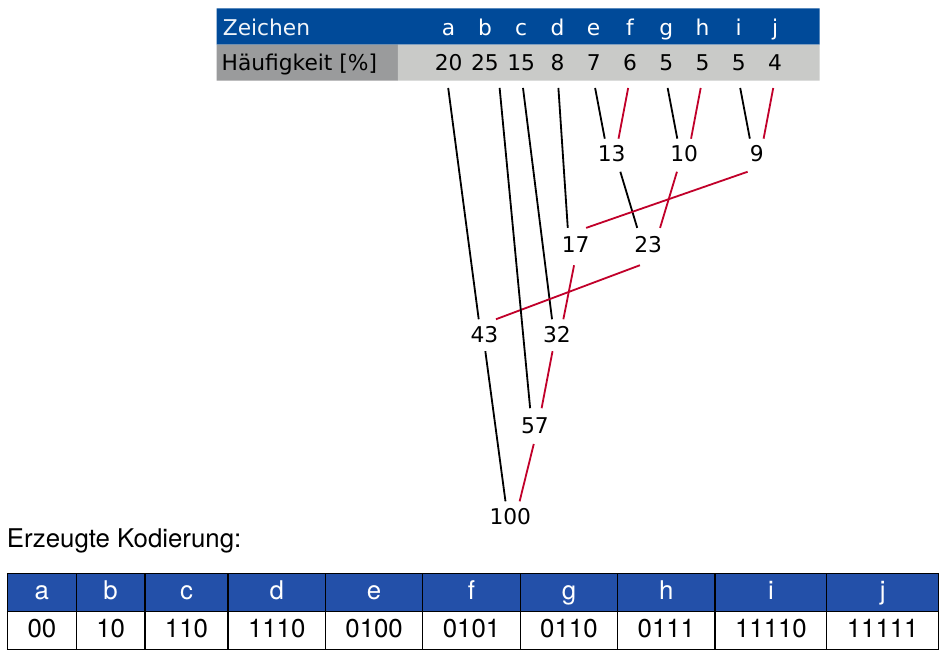
\includegraphics[width=0.8\textwidth, center]{./figures/huffman_codierung.png}
                  \end{minipage}
                }
              }
              child {
                node {Präfixcodes
                  \resizebox{\textwidth}{!}{
                    \begin{minipage}[t]{8cm}
                      \begin{itemize}
                        \item $a_{1}\ldots a_{p}\in A^{*}$ heißt \alert{Präfix} von $b_{1}\ldots b_{l}\in A^{*}$, falls $p\le l$ und $\forall i: a_i=b_i$, $1\le i\le p$
                        \item Ein Code $c:A\rightarrow\{0,1\}^{*}$ heißt \alert{Präfixcode}, falls es kein Paar $i,j\in\{\,1,\ldots,m\}$ gibt, so dass $c(a_i)$ Präfix von $c(a_j)$
                        \item Bei Präfixcodes können Wörter über $\{0, 1\}$ eindeutig dekodiert werden. (Sie entsprechen Binärbäumen mit codierten Zeichen an den Blättern.)
                      \end{itemize}
                    \end{minipage}
                  }
                }
              }
            }
        }
      }
    }
    child {
      node {Kodierung von Zahlen}
      child {
        node {Zahlensysteme}
        child {
          node {Binärsystem / Dualsystem}
        }
        child {
          node {Oktalsystem}
        }
        child {
          node {Dezimalsystem}
        }
        child {
          node {Hexadezimalsystem}
        }
      }
      child {
        node {(Negative) Festkommazahlen
          \resizebox{\textwidth}{!}{
            \begin{minipage}[t]{8cm}
              \begin{itemize}
                \item Bei der Darstellung negativer Festkommazahlen nimmt die höchstwertigste Stelle $d_n$ eine Sonderrolle ein: 
                \begin{itemize}
                  \item Ist $d_n = 0$, so handelt es sich um eine \alert{nichtnegative Zahl}
                \end{itemize}
              \end{itemize}
            \end{minipage}
          }
        }
        child {
          node {Darstellung durch Betrag und Vorzeichen
            \resizebox{\textwidth}{!}{
              \begin{minipage}[t]{10cm}
                \begin{itemize}
                  \item $\displaystyle[d_{n},d_{n-1},\ldots, d_{0}]_{BV}:=\left(-1\right)^{d_{n}}\sum_{i=0}^{n-1}d_i\;2^{i}$
                \end{itemize}
                % \begin{tabular}{>{\centering}m{0.1\textwidth}|>{\centering}m{0.1\textwidth}>{\centering}m{0.1\textwidth}>{\centering}m{0.1\textwidth}>{\centering}m{0.1\textwidth}>{\centering}m{0.1\textwidth}>{\centering}m{0.1\textwidth}>{\centering}m{0.1\textwidth}>{\centering}m{0.1\textwidth}m{0pt}}
                %   % \toprule
                %   d & 000 & 001 & 010 & 011 & 100 & 101 & 110 & 111 &\\
                %   % \hlineB{4}
                %   \hline
                %   $[d]_{BV}$ & 0 & 1 & 2 & 3 & 0 & -1 & -2 & -3 &\\
                %   % \bottomrule
                % \end{tabular}
              \end{minipage}
            }
          }
        }
        child {
          node {Einer-Komplement-Darstellung
            \resizebox{\textwidth}{!}{
              \begin{minipage}[t]{8cm}
                \begin{itemize}
                  \item $\displaystyle[d_{n},d_{n-1},\ldots, d_{0}]_{1}:=\sum_{i=0}^{n-1}d_i\;2^i-d_n(2^n-1)$
                \end{itemize}
              \end{minipage}
            }
          }
        }
        child {
          node {Zweier-Komplement-Darstellung
            \resizebox{\textwidth}{!}{
              \begin{minipage}[t]{8cm}
                \begin{itemize}
                  \item $\displaystyle[d_{n},d_{n-1},\ldots, d_{0}]_{2}:=\sum_{i=0}^{n-1}d_i\;2^i-d_n\;2^n$
                \end{itemize}
              \end{minipage}
            }
          }
        }
      }
      child {
        node {Gleitkommazahlen}
      }
    }
    child {
      node {Mathematische Grundlagen}
    }
    child {
      node {RETI-Maschine}
    };
  \end{scope}
  % ┌───────────────────┐
  % │ Verbindungslinien │
  % └───────────────────┘
  \begin{pgfonlayer}{background}
  % \draw [concept connection]
  %     (datahazardsforbranches) edge (forwarding);
  \end{pgfonlayer}
  % ┌──────────────┐
  % │ Annotationen │
  % └──────────────┘
  % https://tex.stackexchange.com/questions/302976/node-positioning-middle-point-mind-map-connection-bar
  \node [annotation, below] at (ca.south) {This mindmap is provided without guarantee of correctness and completeness!};
  \end{tikzpicture}
\end{document}
